\documentclass[aspectratio=169,xcolor=table]{beamer}
\usepackage{algorithm}
\usepackage{algpseudocode}
\usepackage[utf8]{inputenc}
\usepackage[T1]{fontenc}
\usepackage{lipsum, lmodern}
\usepackage{csquotes}
\usepackage{xcolor}
\usepackage[portuguese]{babel}

% ------------------------------------------------
% Tema e Configurações do Beamer
% ------------------------------------------------
\usetheme{DCC}

% Ajuste de espaçamento entre itens
\setbeamertemplate{itemize items}[circle]
\setbeamertemplate{itemize subitem}[circle]
\setlength{\itemsep}{0.8em}
\setlength{\parskip}{0.5em}

\graphicspath{{imgs/}{./imgs/}}

\author[Sena, Luis Felipe; Daniel, João]{%
  \textbf{Luis Felipe Sena} \and \textbf{João Daniel}
}
\title{Inteligência Artificial Distribuída: Técnicas e Aplicações em Sistemas Distribuídos}
\institute{Universidade Federal da Bahia \\ Instituto de Computação}
\date{\today}

\begin{document}

%-------------------------------------------------
%  SLIDE DE TÍTULO
%-------------------------------------------------
\begin{frame}[plain,noframenumbering]
    \titlepage
\end{frame}

%-------------------------------------------------
%  SLIDE DE AGENDA
%-------------------------------------------------
\begin{frame}{Agenda}
    \tableofcontents
\end{frame}

\setlength{\parskip}{1em}

%=================================================
\section{Introdução}
%=================================================
\begin{frame}{Introdução}
    \begin{itemize}
        \item A Inteligência Artificial Distribuída (IAD) emerge como interseção entre IA e sistemas distribuídos
        \item Resolve problemas complexos através da cooperação de múltiplos agentes
        \item Abordagem distribuída para processamento e conhecimento
        \item Fundamental para sistemas modernos de larga escala
    \end{itemize}
\end{frame}

%=================================================
\section{Classificação da IA}
%=================================================
\begin{frame}{Classificação da Inteligência Artificial}
    \begin{center}
        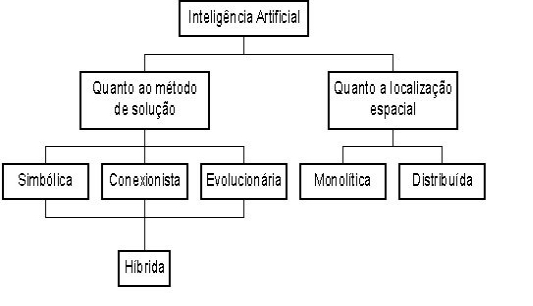
\includegraphics[width=0.7\textwidth]{IAD.jpg}
    \end{center}
\end{frame}

%=================================================
\section{Conceitos Fundamentais}
%=================================================
\begin{frame}{Conceitos Fundamentais da IAD}
    \begin{itemize}
        \item \textbf{Agentes:}
        \begin{itemize}
            \item Autonomia
            \item Inteligência
            \item Mobilidade
            \item Capacidade de comunicação
        \end{itemize}
        \item \textbf{Características dos Sistemas:}
        \begin{itemize}
            \item Descentralização
            \item Cooperação
            \item Coordenação
        \end{itemize}
    \end{itemize}
\end{frame}

%=================================================
\section{Abordagens Principais}
%=================================================
\begin{frame}{Abordagens Principais}
    \vspace{0.5em}
    \begin{columns}[T]
        \begin{column}{0.4\textwidth}
            \textbf{Resolução Distribuída de}\\ \textbf{Problemas (RDP):}
            \vspace{0.5em}
            \begin{itemize}\setlength{\itemsep}{0.5em}
                \item Abordagem top-down
                \item Decomposição em subproblemas
                \item Visão limitada por agente
            \end{itemize}
        \end{column}
        \hfill
        \begin{column}{0.4\textwidth}
            \textbf{Sistemas Multiagentes:}
            \vspace{0.5em}
            \begin{itemize}\setlength{\itemsep}{0.5em}
                \item Abordagem bottom-up
                \item Agentes autônomos
                \item Interação social
            \end{itemize}
        \end{column}
    \end{columns}
\end{frame}

%=================================================
\section{Arquiteturas}
%=================================================
\begin{frame}{Arquiteturas Fundamentais}
    \vspace{0.5em}
    \begin{columns}[T]
        \begin{column}{0.38\textwidth}
            \textbf{Arquitetura Blackboard:}
            \vspace{0.5em}
            \begin{itemize}\setlength{\itemsep}{0.5em}
                \item Espaço compartilhado
                \item Coordenação flexível
                \item Repositório centralizado
            \end{itemize}
        \end{column}
        \hfill
        \begin{column}{0.38\textwidth}
            \textbf{Arquitetura ParaNet:}
            \vspace{0.5em}
            \begin{itemize}\setlength{\itemsep}{0.5em}
                \item Camadas distintas
                \item Tratamento de inconsistências
                \item Coordenação eficiente
            \end{itemize}
        \end{column}
    \end{columns}
\end{frame}

%=================================================
\section{Desafios e Soluções}
%=================================================
\begin{frame}{Desafios e Soluções}
    \begin{itemize}
        \item \textbf{Complexidade:}
        \begin{itemize}
            \item Coordenação entre agentes
            \item Arquiteturas especializadas
        \end{itemize}
        \item \textbf{Inconsistências:}
        \begin{itemize}
            \item Lógica paraconsistente
            \item Tratamento de contradições
        \end{itemize}
        \item \textbf{Comunicação:}
        \begin{itemize}
            \item Protocolos eficientes
            \item Mecanismos de coordenação
        \end{itemize}
    \end{itemize}
\end{frame}

%=================================================
\section{Tendências e Futuro}
%=================================================
\begin{frame}{Tendências e Direções Futuras}
    \begin{itemize}
        \item \textbf{Aprendizado de Máquina Distribuído}
        \item \textbf{Sistemas Multiagentes Autônomos}
        \item \textbf{Aplicações em Larga Escala}
        \begin{itemize}
            \item IoT e Edge Computing
            \item Cidades Inteligentes
            \item Sistemas Autônomos
        \end{itemize}
        \item \textbf{Integração com Tecnologias Emergentes}
        \begin{itemize}
            \item 5G
            \item Computação Quântica
            \item Blockchain
        \end{itemize}
    \end{itemize}
\end{frame}

%=================================================
\section{Aplicações Práticas}
%=================================================
\begin{frame}{Aplicações do Mundo Real}
    \begin{columns}[t]
        \begin{column}{0.38\textwidth}
            \textbf{Áreas de Aplicação:}
            \begin{itemize}
                \item Ensino a Distância
                \item E-commerce
                \item Manufatura
                \item Exploração Espacial
                \item Sistemas de Saúde
            \end{itemize}
        \end{column}
        \begin{column}{0.38\textwidth}
            \textbf{Exemplos Notáveis:}
            \begin{itemize}
                \item Remote Agent (NASA)
                \item Sistemas de Recomendação
                \item HipNav (Cirurgia)
                \item Veículos Autônomos
            \end{itemize}
        \end{column}
    \end{columns}
\end{frame}

%=================================================
\section{Infraestrutura Moderna}
%=================================================
\begin{frame}{Infraestrutura e Componentes Modernos}
    \begin{itemize}
        \item \textbf{Containerização e Orquestração}
        \begin{itemize}
            \item Kubernetes
            \item Docker Swarm
        \end{itemize}
        \item \textbf{Comunicação}
        \begin{itemize}
            \item Apache Kafka
            \item RabbitMQ
        \end{itemize}
        \item \textbf{Armazenamento e Cache}
        \begin{itemize}
            \item Cassandra, MongoDB
            \item Redis, Memcached
        \end{itemize}
    \end{itemize}
\end{frame}

%=================================================
\section{Conclusão}
%=================================================
\begin{frame}{Conclusão}
    \begin{itemize}
        \item IAD é fundamental para sistemas distribuídos modernos
        \item Evolução constante de arquiteturas e padrões
        \item Integração crescente com novas tecnologias
        \item Democratização do uso em diferentes domínios
        \item Futuro promissor com novos desafios e oportunidades
    \end{itemize}
\end{frame}

%=================================================
\section{Referências}
%=================================================
\begin{frame}[allowframebreaks]{Referências}
    \nocite{*}
    \bibliographystyle{plain}
    \bibliography{Bibliografia}
\end{frame}

\end{document}
